\begin{center}
  \normalsize{\cyr{\textbf{№3.5}}}
\end{center}


\begin{figure}[h!]
  \centering
  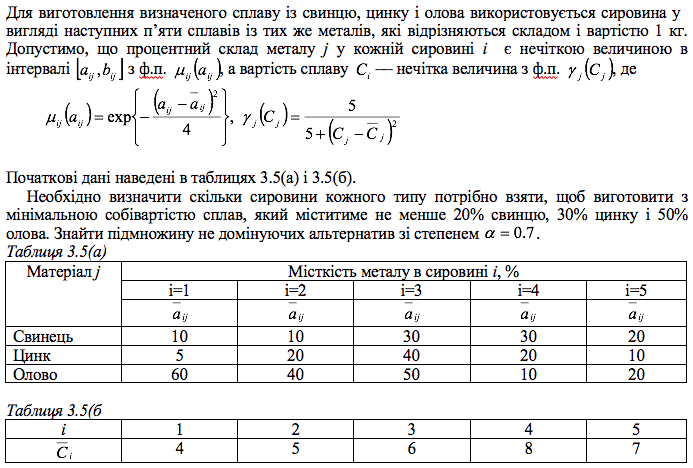
\includegraphics[width=13cm]{3_5.png}
  \centering
\end{figure}


Математична модель: $x_{ij}$ частина вмісту матеріалу $j$  отриманого з сплаву $i$
\Code{
min \quad   \sum_j^3 C_{j} x_{ij} \qquad  \text{Обмеження} \quad  \sum_i^5 a_{ij}  x_{ij} \leqslant b_i
}

\begin{multicols}{2}

  $$\mu(a_{ij}) \geqslant 0.7  $$

  $$ \exp\{ - \dfrac{(a_{ij}-\overline{a}_{ij})^2}{4} \} \geqslant 0.7 $$
  $$- \dfrac{(a_{ij}-\overline{a}_{ij})^2}{4} \geqslant \ln{0.7} $$
  $$ (a_{ij}-\overline{a}_{ij})^2 \leqslant -4 \ln{0.7} $$
  $$ (a_{ij}-\overline{a}_{ij})^2 \leqslant 4 \ln{\dfrac{1}{0.7}} $$
  $$|a_{ij}-\overline{a}_{ij}| \leqslant  \sqrt{4\ln{\dfrac{10}{7}}} $$
  $$ a_{ij} - 2 \sqrt{\ln{\dfrac{10}{7}}} \leqslant a_{ij} \leqslant a_{ij} + 2 \sqrt{ \ln{\dfrac{10}{7}}}$$

  \columnbreak

  $$\gamma(C_{j}) \geqslant 0.7 $$

  $$ \dfrac{5}{5+(C_{j}-\overline{C}_{j})^2} \geqslant 0.7 $$
  $$ \dfrac{5}{0.7} \geqslant 5+(C_{j}-\overline{C}_{j})^2 $$
  $$ \dfrac{5}{0.7}- 5 \geqslant (C_{j}-\overline{C}_{j})^2$$
  $$ \dfrac{15}{7} \geqslant (C_{j}-\overline{C}_{j})^2$$
  $$ \sqrt{\dfrac{15}{7}} \geqslant |C_{j}-\overline{C}_{j}|$$
  $$C_{j} - \sqrt{\dfrac{15}{7}} \leqslant C_{j} \leqslant C_{ij} + \sqrt{\dfrac{15}{7}}$$

\end{multicols}



\begin{multicols}{2}

  \Title{Задача песиміста}

  \Code{
    min \sum_i^5( \overline{C}_{j}  + \sqrt{\dfrac{15}{7}}) x_{ij}
  }

  \Title{Обмеження}

  \Code{
    \sum_j^3( \overline{a}_{ij} + 2 \sqrt{ \ln{\dfrac{10}{7}}} ) x_{ij} \geqslant b_j
  }

  \columnbreak

  \Title{Задача оптиміста}


  \Code{
    min \sum_i^5( \overline{C}_{j} -  \sqrt{\dfrac{15}{7}}) x_{ij}
  }

  \Title{Обмеження}

  \Code{
    \sum_j^3( \overline{a}_{ij} - 2 \sqrt{ \ln{\dfrac{10}{7}}} ) x_{ij} \geqslant b_j
  }

\end{multicols}
